
\documentclass[sigconf,nonacm]{acmart}
\usepackage{pgfplots}
\pgfplotsset{compat=1.18}
\settopmatter{printacmref=false}
\setcopyright{none}

\begin{document}

\title{Detecting LLM-Generated Phishing Emails:
Classical Classifiers vs. LLM-Based Detectors}


\author{Omar Aslan}
\affiliation{%
  \institution{Vistula University}
  \city{Warsaw}
  \country{Poland}
}

\author{Illia Volkov}
\affiliation{%
  \institution{Vistula University}
  \city{Warsaw}
  \country{Poland}
}

\author{Khalid Chalabi}
\affiliation{%
  \institution{Vistula University}
  \city{Warsaw}
  \country{Poland}
}


\begin{abstract}

The increasing use of large language models (LLMs)
in cybercrime has raised concerns about the ability
of existing detection methods to distinguish
human-written phishing emails from AI-generated
phishing content.

This study compares classical machine learning
classifiers with a zero-shot LLM-based detector
for identifying the authorship of phishing emails.

The experimental dataset contains 9,986 phishing
emails, including 5,000 human-written samples and
4,986 emails generated by GPT-4.1, DeepSeek 3.2,
and Llama 3.3 70B.

Three classical classifiers---Logistic Regression,
Support Vector Machine (SVM), and Random Forest---
were implemented using TF-IDF features and evaluated
through a leave-one-generator-out strategy.

Their performance was compared with the pretrained
Qwen2.5-1.5B-Instruct model using zero-shot
classification.

The final evaluation used 400 held-out emails.
Logistic Regression and SVM achieved 100\% accuracy
across all three generator-specific comparisons,
while Random Forest achieved 99--100\%.

In contrast, the zero-shot Qwen detector achieved
29--34.5\% accuracy.

However, additional analysis revealed substantial
dataset bias. All human-written emails were stored
as single-line texts, whereas LLM-generated emails
contained multiple lines.

A simple line-count rule perfectly separated the
classes, indicating that dataset construction could
strongly influence detection performance.

These findings highlight the importance of dataset
quality, controlled evaluation, and external
validation when assessing AI-generated phishing
email detection systems.

\end{abstract}

\keywords{
Phishing Email Detection,
Large Language Models,
Machine Learning,
AI-Generated Text Detection,
TF-IDF,
Dataset Bias,
Cybersecurity
}

\maketitle

\section{Introduction}

Phishing remains an important cybersecurity threat
that relies on deceptive communication to manipulate
recipients into revealing sensitive information or
performing harmful actions.

The development of large language models has
introduced new possibilities for producing
convincing phishing messages at scale.

These technologies can generate fluent and
contextually appropriate emails, raising questions
about the effectiveness of existing detection
approaches.

An important distinction exists between detecting
whether an email is malicious and identifying
whether its content was written by a human or
generated by a language model.

This study focuses specifically on the second task:
distinguishing human-written phishing emails from
LLM-generated phishing emails.

To investigate this problem, three classical machine
learning classifiers are compared with a pretrained
LLM-based detector.

The classical approaches include Logistic Regression,
Support Vector Machine, and Random Forest.
These classifiers use Term Frequency-Inverse Document
Frequency (TF-IDF) text representations.

The LLM-based approach uses Qwen2.5-1.5B-Instruct
with zero-shot classification.

The study evaluates classification performance
across phishing emails generated by GPT-4.1,
DeepSeek 3.2, and Llama 3.3 70B.

In addition to comparing classification accuracy,
the research examines cross-generator generalization,
computational efficiency, and potential dataset bias.

Particular attention is given to determining whether
high classification scores reflect meaningful
authorship differences or systematic characteristics
introduced during dataset construction.

The study contributes an experimental comparison of
the selected detection approaches and an analysis
of dataset artifacts that may affect the reliability
of reported detection performance.


\section{Related Work}

\subsection{Classical Machine Learning and
Transformer-Based Phishing Detection}

Tarapiah et al.~\cite{tarapiah2025} compared
traditional machine learning algorithms with
fine-tuned transformer-based models for phishing
email and URL detection.

Their evaluation included Logistic Regression,
Support Vector Machines, Random Forest,
DistilBERT, and other transformer models.

Random Forest achieved high classification
accuracy, while transformer-based approaches
also demonstrated strong detection capabilities.

However, the primary classification task was
detecting phishing rather than determining
whether a phishing email was written by a
human or generated by an LLM.

\subsection{Dataset Quality and Benchmark Limitations}

Pajola et al.~\cite{pajola2025} investigated
limitations in existing phishing email
detection benchmarks.

Their study demonstrated that near-perfect
performance on familiar datasets does not
necessarily indicate reliable performance
on more challenging evaluation data.

The authors introduced E-PhishGEN, a framework
for generating phishing email datasets,
and evaluated detection methods using a
new multilingual benchmark.

Their findings emphasize the importance of
representative datasets and evaluations
across different data distributions.

\subsection{Detection of LLM-Generated
Phishing Emails}

Gutierrez et al.~\cite{gutierrez2026}
investigated the detection of phishing emails
generated by different large language models.

Their dataset contained 9,986 phishing emails,
including 5,000 human-written samples and
4,986 emails generated by GPT-4.1,
DeepSeek 3.2, and Llama 3.3 70B.

Using stylometric features and supervised
classifiers, the authors examined detection
performance across different generators.

Their results highlighted the importance
of evaluating cross-generator generalization
and adapting detection thresholds.

The publicly released dataset from this
research forms the basis of our experiments.

\subsection{Synthesis and Research Gap}

The three studies demonstrate that machine
learning and transformer-based approaches
can achieve strong performance in
phishing-related classification tasks.

However, detecting malicious emails is
different from identifying the authorship
of emails already known to be phishing.

Furthermore, high accuracy on a single
dataset may reflect source-specific,
formatting, or topic-related patterns.

Our study extends this discussion by
comparing supervised TF-IDF classifiers
with a zero-shot LLM detector on the
human-versus-LLM phishing authorship task.

We additionally investigate structural
dataset artifacts that may affect
the interpretation of detection accuracy.


\section{Research Gap and Methodology}

\subsection{Research Gap}

Existing phishing detection research has
demonstrated strong performance using
classical machine learning and
transformer-based approaches.

However, conventional phishing detection
focuses primarily on distinguishing malicious
emails from legitimate communications.

Identifying whether a phishing email was
written by a human or generated by an LLM
is a different classification problem.

Furthermore, high classification accuracy
may be influenced by dataset-specific
formatting, vocabulary, and source
characteristics.

This study addresses these concerns by
comparing supervised classical classifiers
with a zero-shot LLM-based detector and
investigating potential dataset bias.

\subsection{Research Questions}

The study investigates three research
questions:

\begin{enumerate}
    \item How accurately can classical
    machine learning classifiers distinguish
    human-written phishing emails from
    LLM-generated phishing emails?

    \item How does a zero-shot LLM detector
    perform compared with supervised
    classical classifiers?

    \item To what extent can dataset
    formatting and source-related
    characteristics influence classification
    performance?
\end{enumerate}

\subsection{Dataset Description}

The experiments used the publicly available
dataset associated with the research of
Gutierrez et al.~\cite{gutierrez2026}.

The dataset contains 9,986 phishing emails:
5,000 human-written samples and 4,986
LLM-generated samples.

The synthetic emails were produced using
GPT-4.1, DeepSeek 3.2, and
Llama 3.3 70B.

The classification labels were defined as
follows:

\begin{itemize}
    \item Class 0: Human-written phishing emails.
    \item Class 1: LLM-generated phishing emails.
\end{itemize}

The data were divided using stratified
sampling into 6,989 training samples,
999 validation samples, and
1,998 test samples.

A random state of 42 was used to support
reproducibility.

\subsection{Text Preprocessing}

Email texts were normalized before
classification.

Preprocessing included converting text
to lowercase, removing URLs and email
addresses, removing numerical sequences,
and normalizing whitespace.

For classical machine learning, the
normalized texts were converted into
TF-IDF feature representations.

The same text normalization function
was used for the zero-shot LLM detector.

\subsection{Experimental Design}

Three supervised classifiers were evaluated:
Logistic Regression, Support Vector Machine,
and Random Forest.

The LLM-based detector used the pretrained
Qwen2.5-1.5B-Instruct model without
task-specific fine-tuning.

To assess cross-generator performance,
a leave-one-generator-out strategy was
used for the classical classifiers.

For each experiment, the target LLM
generator was excluded from training.

The final evaluation selected 400 emails
from the reserved test partition:
100 human-written emails and 100 emails
from each LLM generator.

Each generator-specific experiment paired
100 human-written emails with 100
LLM-generated emails.

The same human-written test emails were
reused across the three comparisons.

Performance was measured using accuracy,
precision, recall, F1-score, and
confusion matrices.

Additional experiments examined structural
features and dataset biases to evaluate
the reliability of the classification
results.


\section{Implementation}

\subsection{Development Environment}

The experimental framework was implemented
using Python in Google Colab.

Pandas was used for dataset processing,
Scikit-learn for classical machine learning,
and PyTorch with Hugging Face Transformers
for the LLM-based detector.

An NVIDIA T4 GPU was used for inference
with the pretrained language model.

\subsection{Classical Machine Learning Models}

Three supervised classifiers were implemented:
Logistic Regression, Support Vector Machine
(SVM), and Random Forest.

The email texts were converted into numerical
features using Term Frequency-Inverse Document
Frequency (TF-IDF).

The vectorizer was configured with a maximum
of 30,000 features, unigram and bigram
representations, and a minimum document
frequency of two.

Logistic Regression used a maximum of
1,000 iterations.

The linear SVM was implemented using
LinearSVC with a maximum of 5,000 iterations.

Random Forest used 100 decision trees
and a minimum leaf size of two.

A random state of 42 was used for
reproducibility.

The TF-IDF vectorizer was fitted only
on the training data in each experiment.

\subsection{LLM-Based Detector}

The LLM-based detector used the pretrained
Qwen2.5-1.5B-Instruct model.

Unlike the classical classifiers, Qwen
was evaluated using zero-shot classification
without task-specific fine-tuning.

The model received an instruction to
determine whether each phishing email
was written by a human or generated
by a large language model.

The permitted output labels were
\texttt{HUMAN} and \texttt{LLM}.

The prompt explicitly stated that all
samples were phishing emails and instructed
the detector to ignore instructions
embedded in the email content.

Input sequences were truncated to a
maximum of 1,536 tokens.

Deterministic generation was used by
disabling sampling and limiting output
to eight new tokens.

Predictions and inference times were
recorded for subsequent evaluation.

\subsection{Experimental Pipeline}

The implementation followed a consistent
experimental procedure.

First, the original dataset was divided
into training, validation, and testing
partitions.

Second, the classical classifiers were
trained using normalized email text
and TF-IDF representations.

Third, leave-one-generator-out experiments
were performed by excluding the target
LLM generator from training.

Fourth, the trained classifiers were
evaluated on held-out human-written and
LLM-generated phishing emails.

The zero-shot Qwen detector was evaluated
on the same final test samples.

The final evaluation included 400 unique
emails, consisting of 100 human-written
samples and 100 samples from each of
the three LLM generators.

Each generator-specific comparison used
a balanced set of 200 emails.

\subsection{Reproducibility}

Model configurations and random states
were kept consistent throughout the
final experiments.

Exact text overlap between training
and test partitions was checked.

The final test dataset was saved with
a SHA-256 fingerprint.

Predictions, classification metrics,
and execution times were stored in
CSV files.

The implementation therefore supports
reproducible evaluation under the
documented experimental conditions.

Nevertheless, exact computational results
may vary with hardware, software versions,
and runtime environments.


\section{Experimental Results}

\subsection{Final Classification Performance}

The final evaluation compared three supervised
classical machine learning classifiers with
the zero-shot Qwen2.5-1.5B-Instruct detector.

Three generator-specific experiments were
conducted using GPT-4.1, DeepSeek 3.2,
and Llama 3.3 70B.

Each evaluation contained 200 emails,
including 100 human-written phishing emails
and 100 emails from the target generator.

The classical classifiers were trained
without samples from the target generator.

All four detectors were evaluated using
the same test examples within each
generator-specific comparison.

Table~\ref{tab:final_results} presents the
final accuracy, precision, recall,
and F1-score results.
Figure~\ref{fig:accuracy} compares the
classification accuracy of the four detectors.

Figure~\ref{fig:f1} presents the corresponding
F1-score results across the three generators.
\begin{table*}[t]
\centering
\caption{Final Classification Performance
Across LLM Generators (\%)}
\label{tab:final_results}
\small
\begin{tabular}{llrrrr}
\toprule
Generator & Detector & Accuracy &
Precision & Recall & F1-score \\
\midrule
GPT-4.1 & Logistic Regression &
100.00 & 100.00 & 100.00 & 100.00 \\
GPT-4.1 & SVM &
100.00 & 100.00 & 100.00 & 100.00 \\
GPT-4.1 & Random Forest &
100.00 & 100.00 & 100.00 & 100.00 \\
GPT-4.1 & Qwen2.5-1.5B &
34.00 & 38.57 & 54.00 & 45.00 \\
\midrule
DeepSeek 3.2 & Logistic Regression &
100.00 & 100.00 & 100.00 & 100.00 \\
DeepSeek 3.2 & SVM &
100.00 & 100.00 & 100.00 & 100.00 \\
DeepSeek 3.2 & Random Forest &
100.00 & 100.00 & 100.00 & 100.00 \\
DeepSeek 3.2 & Qwen2.5-1.5B &
34.50 & 39.01 & 55.00 & 45.64 \\
\midrule
Llama 3.3 & Logistic Regression &
100.00 & 100.00 & 100.00 & 100.00 \\
Llama 3.3 & SVM &
100.00 & 100.00 & 100.00 & 100.00 \\
Llama 3.3 & Random Forest &
99.00 & 100.00 & 98.00 & 98.99 \\
Llama 3.3 & Qwen2.5-1.5B &
29.00 & 33.85 & 44.00 & 38.26 \\
\bottomrule
\end{tabular}
\end{table*}

Logistic Regression and SVM achieved
100\% accuracy across all three
generator-specific test sets.

Random Forest achieved 100\% accuracy
for GPT-4.1 and DeepSeek 3.2,
and 99\% for Llama 3.3.

In contrast, Qwen achieved accuracies
of 34\%, 34.5\%, and 29\%, respectively.

These results demonstrate substantially
higher performance for the supervised
classifiers under the evaluated conditions.

However, the two approaches used different
training protocols: supervised learning
for classical classifiers and zero-shot
inference for Qwen.

Therefore, these results do not establish
the general superiority of classical
machine learning over LLM-based detectors.


\subsection{Classification Error Analysis}

Confusion matrices were examined to
investigate the classification errors
produced by the zero-shot detector.

The positive class represented
LLM-generated phishing emails.

Table~\ref{tab:qwen_errors} summarizes
the Qwen confusion matrix results.

\begin{table}[t]
\centering
\caption{Qwen Confusion Matrix Results}
\label{tab:qwen_errors}
\small
\begin{tabular}{lrrrr}
\toprule
Generator & TN & FP & FN & TP \\
\midrule
GPT-4.1 & 14 & 86 & 46 & 54 \\
DeepSeek 3.2 & 14 & 86 & 45 & 55 \\
Llama 3.3 & 14 & 86 & 56 & 44 \\
\bottomrule
\end{tabular}
\end{table}

Qwen incorrectly classified 86 of the
100 human-written phishing emails as
LLM-generated in each comparison.

It also failed to identify 46 GPT-4.1,
45 DeepSeek 3.2, and 56 Llama 3.3
generated emails.

These findings demonstrate a substantial
false-positive tendency under the selected
zero-shot prompt configuration.

The same 100 human-written emails were
used across the three evaluations;
therefore, the reported false positives
are not independent observations.


% Figure 1: Accuracy Comparison

\begin{figure*}[t]
\centering
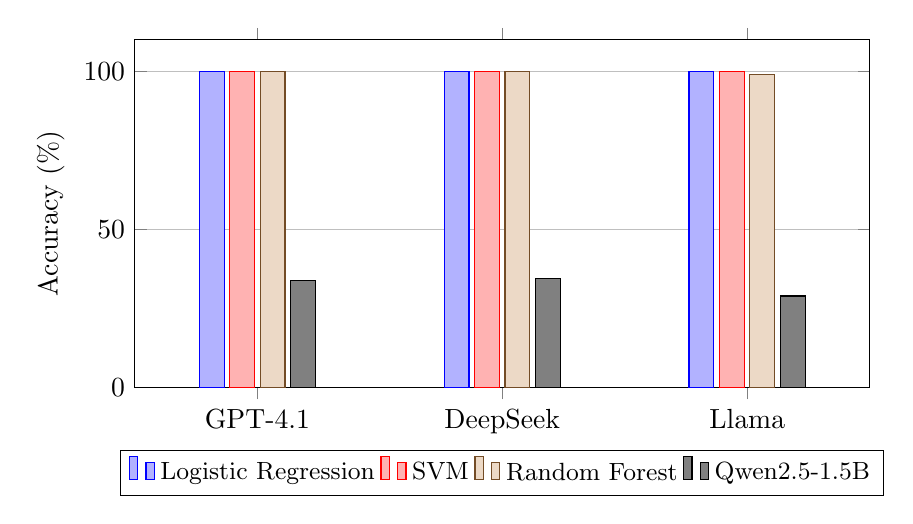
\begin{tikzpicture}
\begin{axis}[
    ybar,
    bar width=9pt,
    width=0.9\textwidth,
    height=6cm,
    ymin=0,
    ymax=110,
    ylabel={Accuracy (\%)},
    symbolic x coords={
        GPT-4.1,
        DeepSeek,
        Llama
    },
    xtick=data,
    ymajorgrids=true,
    enlarge x limits=0.25,
    legend style={
        at={(0.5,-0.18)},
        anchor=north,
        legend columns=4,
        font=\small
    }
]

\addplot coordinates {
    (GPT-4.1,100)
    (DeepSeek,100)
    (Llama,100)
};

\addplot coordinates {
    (GPT-4.1,100)
    (DeepSeek,100)
    (Llama,100)
};

\addplot coordinates {
    (GPT-4.1,100)
    (DeepSeek,100)
    (Llama,99)
};

\addplot coordinates {
    (GPT-4.1,34)
    (DeepSeek,34.5)
    (Llama,29)
};

\legend{
    Logistic Regression,
    SVM,
    Random Forest,
    Qwen2.5-1.5B
}

\end{axis}
\end{tikzpicture}

\caption{Final classification accuracy
across three LLM generators.
Each comparison contains 100 human-written
and 100 LLM-generated phishing emails.}

\Description{Grouped bar chart comparing accuracy
across GPT-4.1, DeepSeek 3.2, and Llama 3.3.
Logistic Regression and SVM achieve 100 percent
accuracy on all three groups. Random Forest
achieves 100, 100, and 99 percent. Qwen achieves
34, 34.5, and 29 percent, respectively.}

\label{fig:accuracy}
\end{figure*}


% Figure 2: F1-score Comparison

\begin{figure*}[t]
\centering
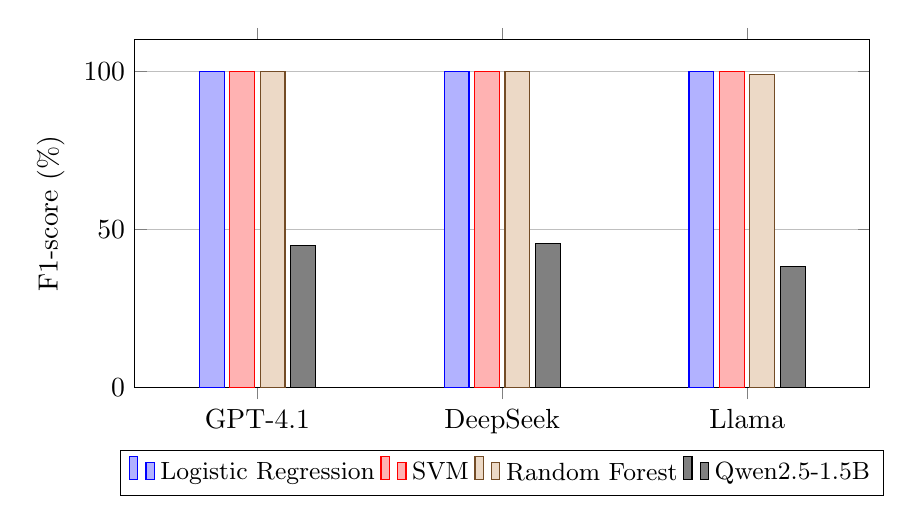
\begin{tikzpicture}
\begin{axis}[
    ybar,
    bar width=9pt,
    width=0.9\textwidth,
    height=6cm,
    ymin=0,
    ymax=110,
    ylabel={F1-score (\%)},
    symbolic x coords={
        GPT-4.1,
        DeepSeek,
        Llama
    },
    xtick=data,
    ymajorgrids=true,
    enlarge x limits=0.25,
    legend style={
        at={(0.5,-0.18)},
        anchor=north,
        legend columns=4,
        font=\small
    }
]

\addplot coordinates {
    (GPT-4.1,100)
    (DeepSeek,100)
    (Llama,100)
};

\addplot coordinates {
    (GPT-4.1,100)
    (DeepSeek,100)
    (Llama,100)
};

\addplot coordinates {
    (GPT-4.1,100)
    (DeepSeek,100)
    (Llama,98.99)
};

\addplot coordinates {
    (GPT-4.1,45)
    (DeepSeek,45.64)
    (Llama,38.26)
};

\legend{
    Logistic Regression,
    SVM,
    Random Forest,
    Qwen2.5-1.5B
}

\end{axis}
\end{tikzpicture}

\caption{Final F1-score comparison across
three LLM generators using the same
balanced evaluation samples.}

\Description{Grouped bar chart comparing F1-scores
for four classifiers across three LLM generators.
Logistic Regression and SVM achieve 100 percent
on all three groups. Random Forest achieves
100, 100, and 98.99 percent. Qwen achieves
45, 45.64, and 38.26 percent, respectively.}

\label{fig:f1}
\end{figure*}

\subsection{Dataset Bias Analysis}

Additional experiments were conducted to
investigate whether dataset-specific
characteristics influenced classification
performance.

\subsubsection{Formatting Bias}

A substantial formatting difference was
identified between the two classes.

All 5,000 human-written phishing emails
were stored as single-line texts.

In contrast, all 4,986 LLM-generated emails
contained multiple lines, ranging from
9 to 31 lines, with a median of 17.

A simple classification rule based only
on whether an email contained more than
one line achieved 100\% accuracy on
an examined sample of 200 emails.

This finding demonstrates that formatting
characteristics alone could distinguish
the two classes in the original dataset.

\subsubsection{Feature Ablation Analysis}

To investigate the influence of structural
characteristics, a Logistic Regression
classifier was evaluated using six
numerical email features:

character count, word count, line count,
digit count, exclamation mark count,
and URL count.

Selected features were progressively
removed to examine their contribution
to classification performance.

Table~\ref{tab:ablation} presents the
results of these experiments.

\begin{table}[t]
\centering
\caption{Structural Feature Ablation Results}
\label{tab:ablation}
\footnotesize
\begin{tabular}{p{0.49\columnwidth}rr}
\toprule
Feature Configuration &
Accuracy (\%) & F1 (\%) \\
\midrule
All six features & 100.00 & 100.00 \\
Line count only & 100.00 & 100.00 \\
Without line count & 89.19 & 79.78 \\
Without lines, digits,
and URLs & 58.41 & 54.52 \\
\bottomrule
\end{tabular}
\end{table}

The results demonstrate that line count
was a particularly strong predictor.

Removing line count reduced accuracy
from 100\% to 89.19\%.

Further removal of digit and URL counts
reduced accuracy to 58.41\%.

These findings suggest that numerical
classifiers can achieve high performance
by exploiting structural characteristics
of the dataset.

However, these experiments were separate
from the final TF-IDF-based evaluation.

The TF-IDF models used normalized texts
with line breaks removed.

Therefore, their high accuracy cannot
be attributed directly to line count.

\subsubsection{Source and Topic Bias}

The two classes also originated from
different collection and generation
processes.

Human-written samples were collected
from TREC-07, CEAS\_08, Nazario,
Nigerian\_Fraud, and
enron\_data\_fraud\_labeled.

In contrast, the synthetic emails were
generated using GPT-4.1, DeepSeek 3.2,
and Llama 3.3 70B.

Furthermore, category metadata was missing
for all human-written samples, while
synthetic samples were associated with
five phishing topics.

Neither source nor category metadata
was directly supplied to the final
classifiers as an input feature.

Nevertheless, source-related vocabulary
and topic differences may remain
detectable within the email texts.

\subsubsection{Implications}

The dataset bias analysis highlights
an important limitation of interpreting
near-perfect classification accuracy.

Although the final classifiers performed
well on held-out test samples, these
samples originated from the same broader
data collection and generation processes.

Consequently, additional evaluation on
independently collected, topic-matched,
and formatting-controlled datasets is
necessary to establish whether the
detectors learn generalizable
authorship-related patterns.

\subsection{Computational Efficiency Analysis}

Computational efficiency was evaluated
using the recorded training and inference
times of the four detection approaches.

The measurements included classifier
training time, average inference latency
per email, and total inference time
for each generator-specific test set.

\subsubsection{Classical Machine Learning}

The classical classifiers demonstrated
relatively short training and prediction
times.

Logistic Regression required approximately
3.06--3.92 seconds for training.

Linear SVM required 2.63--2.72 seconds,
while Random Forest required
4.20--5.63 seconds.

SVM achieved the lowest average inference
latency, approximately
0.29--0.35 milliseconds per email.

Logistic Regression required
0.68--0.75 milliseconds per email,
whereas Random Forest required
0.81--0.98 milliseconds per email.

The classical training times included
TF-IDF vectorizer fitting and classifier
training.

\subsubsection{LLM-Based Detector}

Qwen2.5-1.5B-Instruct was used without
task-specific fine-tuning.

Therefore, task-specific training time
was not applicable.

Its average inference latency ranged
from approximately 173 to 176
milliseconds per email.

The total recorded inference time
for all 400 unique test emails
was 65.97 seconds.

Table~\ref{tab:efficiency} presents
the detailed measurements.

\begin{table*}[t]
\centering
\caption{Computational Efficiency
Comparison Across LLM Generators}
\label{tab:efficiency}
\footnotesize
\begin{tabular}{llrrr}
\toprule
Generator & Detector &
Training (s) &
Inference (ms/email) &
Total Inference (s) \\
\midrule
GPT-4.1 & Logistic Regression &
3.9150 & 0.7110 & 0.1422 \\
GPT-4.1 & SVM &
2.6770 & 0.2858 & 0.0572 \\
GPT-4.1 & Random Forest &
5.6298 & 0.8113 & 0.1623 \\
GPT-4.1 & Qwen2.5-1.5B &
N/A & 172.9980 & 34.5996 \\
\midrule
DeepSeek 3.2 & Logistic Regression &
3.0551 & 0.7461 & 0.1492 \\
DeepSeek 3.2 & SVM &
2.7224 & 0.3510 & 0.0702 \\
DeepSeek 3.2 & Random Forest &
4.7371 & 0.9800 & 0.1960 \\
DeepSeek 3.2 & Qwen2.5-1.5B &
N/A & 175.5733 & 35.1147 \\
\midrule
Llama 3.3 & Logistic Regression &
3.2116 & 0.6799 & 0.1360 \\
Llama 3.3 & SVM &
2.6312 & 0.3504 & 0.0701 \\
Llama 3.3 & Random Forest &
4.1988 & 0.8219 & 0.1644 \\
Llama 3.3 & Qwen2.5-1.5B &
N/A & 175.6803 & 35.1361 \\
\bottomrule
\end{tabular}
\end{table*}

\subsubsection{Interpretation}

The classical machine learning models
demonstrated substantially lower measured
inference latency than the zero-shot
LLM-based detector.

SVM was the fastest classifier under
the evaluated conditions while also
achieving 100\% accuracy across
the generator-specific final tests.

However, the execution conditions
were not hardware-equivalent.

The classical classifiers used
CPU-based batch predictions,
whereas Qwen performed sequential
generation on an NVIDIA T4 GPU.

Additionally, Qwen model loading time
was excluded from the measurements.

The same 100 human-written test emails
were reused in each generator-specific
evaluation.

Therefore, the three Qwen test-set
inference times should not be summed
to obtain the runtime of 400 unique emails.

These results represent implementation-
specific efficiency rather than a
standardized hardware benchmark.

\section{Discussion and Limitations}

\subsection{Interpretation of the Results}

The experiments revealed substantial
differences between supervised classical
machine learning classifiers and the
zero-shot LLM-based detector.

Logistic Regression and SVM achieved
100\% accuracy across all three
generator-specific final test sets.

Random Forest achieved 99--100\%
accuracy, while Qwen2.5-1.5B-Instruct
achieved only 29--34.5\%.

These findings indicate that the
supervised classifiers were highly
effective at separating the two classes
within the selected dataset.

However, near-perfect performance should
not automatically be interpreted as
evidence of generalizable authorship
detection.

The dataset bias experiments identified
systematic differences that may have
contributed to classification performance.

\subsection{Dataset Bias and Validity}

The most significant limitation
concerns dataset construction.

All human-written phishing emails
were represented as single-line texts,
whereas the LLM-generated emails
contained multiple lines.

A simple line-count rule achieved
100\% accuracy on the examined samples.

Furthermore, human-written emails
originated from existing email corpora,
while synthetic emails were generated
using a separate process.

These differences create potential
formatting, vocabulary, and topic
confounding factors.

Although the final TF-IDF classifiers
used normalized texts without line
breaks, other dataset-specific
patterns may still have influenced
their predictions.

Therefore, the results establish
performance on the selected dataset,
not reliable authorship detection
across independent real-world sources.

\subsection{Differences in Training Conditions}

The evaluated methods used different
training protocols.

The classical classifiers were trained
on labeled examples of human-written
and LLM-generated phishing emails.

In contrast, Qwen was evaluated
without task-specific fine-tuning,
using only zero-shot instructions.

Consequently, the observed performance
gap does not demonstrate that classical
machine learning is inherently superior
to all LLM-based detection approaches.

Different language models, prompt
strategies, few-shot examples, or
fine-tuning procedures might produce
different results.

\subsection{Experimental Limitations}

Several additional limitations
should be considered.

First, the final evaluation used
400 emails from a single broader
dataset rather than an independently
collected external benchmark.

Second, the same 100 human-written
emails were reused across the three
generator-specific comparisons.

Therefore, these comparisons were
not statistically independent.

Third, only one pretrained LLM-based
detector was evaluated.

Fourth, no confidence intervals or
formal statistical significance tests
were performed.

Finally, computational efficiency
measurements were obtained using
different inference procedures and
hardware configurations.

Classical classifiers used CPU-based
batch inference, whereas Qwen used
sequential GPU-based generation.

These differences limit direct
comparisons of computational efficiency.

\subsection{Future Research Directions}

Future research should evaluate
authorship detection using independently
collected, topic-matched, and
formatting-controlled phishing emails.

Such datasets would help determine
whether classifiers learn genuine
authorship-related characteristics
rather than source-specific patterns.

Additional experiments should examine
larger LLM-based detectors, alternative
prompts, few-shot methods, and
task-specific fine-tuning.

Future studies should also investigate
robustness to paraphrasing, manual
editing, and formatting changes.

Finally, repeated evaluations,
confidence intervals, and standardized
hardware benchmarks would strengthen
the reliability of model comparisons.

\section{Conclusion}

This study investigated the detection of
LLM-generated phishing emails by comparing
three classical machine learning classifiers
with a zero-shot LLM-based detector.

The experiments used 9,986 phishing emails,
including human-written samples and
synthetic emails generated by GPT-4.1,
DeepSeek 3.2, and Llama 3.3 70B.

Logistic Regression, Support Vector Machine,
and Random Forest were implemented using
TF-IDF text representations.

Their performance was compared with
Qwen2.5-1.5B-Instruct, which was evaluated
without task-specific fine-tuning.

The final evaluation used 400 held-out
emails in three generator-specific
comparisons.

Logistic Regression and SVM achieved
100\% accuracy across all three comparisons,
while Random Forest achieved 99--100\%.

In contrast, the zero-shot Qwen detector
achieved accuracies between 29\% and 34.5\%.

The classical classifiers also demonstrated
lower measured inference latency under
the implemented experimental conditions.

However, the most significant finding
concerned dataset validity.

All human-written emails were stored
as single-line texts, whereas the
LLM-generated emails contained multiple
lines.

A simple line-count rule achieved
100\% accuracy on an examined sample,
revealing a strong structural artifact.

Additional feature ablation experiments
confirmed that formatting-related
characteristics could substantially
influence classification performance.

Although the final TF-IDF classifiers
did not directly use line counts,
differences in data sources, topics,
and generation procedures remained
potential confounding factors.

Therefore, the near-perfect accuracy
of classical classifiers should not
be interpreted as proof of reliable
authorship detection in real-world
phishing emails.

The findings demonstrate the importance
of evaluating both classification
performance and dataset quality.

Future research should employ
independently collected, topic-matched,
and formatting-controlled datasets,
together with broader comparisons
of supervised and LLM-based detectors.

Overall, reliable detection of
LLM-generated phishing emails requires
not only effective classification models
but also rigorous evaluation methods
that distinguish genuine authorship
signals from dataset-specific artifacts.

\begin{thebibliography}{3}

\bibitem{tarapiah2025}
Saed Tarapiah, Linda Abbas, Oula Mardawi,
Shadi Atalla, Yassine Himeur, and
Wathiq Mansoor. 2025.
Evaluating the Effectiveness of Large
Language Models (LLMs) Versus Machine
Learning (ML) in Identifying and
Detecting Phishing Email Attempts.
\emph{Algorithms} 18, 10 (2025), 599.
\url{https://doi.org/10.3390/a18100599}

\bibitem{pajola2025}
Luca Pajola, Eugenio Caripoti,
Stefan Banzer,Simeone Pizzi, Mauro Conti, and Giovanni Apruzzese.
2025.
E-PhishGen: Unlocking Novel Research
in Phishing Email Detection.
In \emph{Proceedings of the ACM Workshop
on Artificial Intelligence and Security
(AISec '25)}.
\url{https://doi.org/10.1145/3733799.3762967}

\bibitem{gutierrez2026}
Rommel Gutierrez, William Villegas-Ch,
and Jaime Govea. 2026.
Cross-model evaluation of phishing
detectors against LLM-generated emails.
\emph{Frontiers in Big Data} 9 (2026),
Article 1883452.
\url{https://doi.org/10.3389/fdata.2026.1883452}

\end{thebibliography}


\end{document}
